\documentclass[12pt]{article}

\usepackage[a4paper, margin=1in]{geometry}
\usepackage{graphicx}
\usepackage[absolute, overlay]{textpos}
\usepackage{fancyhdr}
\usepackage{siunitx}
\usepackage{tikz}
\usepackage{pgfplots}
\usetikzlibrary{decorations.pathmorphing}
\usetikzlibrary{math}
\usetikzlibrary{calc}

\pgfplotsset{compat=1.18}

\pagestyle{fancy} %for footers

\newcommand{\customsubject}{}   
\newcommand{\customtitle}{}

\newcounter{questionpartcounter}                  %Setup for question part counter for a,b,c listing
\renewcommand{\thequestionpartcounter}
{\alph{questionpartcounter}}

\newcounter{questionpartpartcounter}                  %Setup for question part  partcounter for a,b,c listing
\renewcommand{\thequestionpartpartcounter}
{\roman{questionpartcounter}}

\pagestyle{fancy} %for footers
\renewcommand{\headrulewidth}{0pt}
\fancyhf{}
\fancyfoot[R]{\thepage}

\newenvironment{worksheet}[2]
{
    
    \global\renewcommand{\customtitle}{#1}
    \global\renewcommand{\customsubject}{#2}


    \begin{textblock*}{5cm}(0.4cm,0.4cm)
   
\includegraphics[width=4cm]{include/figures/bmdwlogo}
\end{textblock*}

    \vspace*{-1cm}
    
    {\large\textbf{\begin{center}\customtitle\end{center}}}

    \begin{center}\customsubject\end{center}
    
    \vspace{0.3cm}
    
    \hspace*{-1.5cm}\textbf{Name:\ \rule{4cm}{0.4pt}}\; 
    \textbf{Student \#: \ \rule{3cm}{0.4pt}}\;
    \textbf{Student Email \#: \ \rule{1.53cm}{0.4pt}}

    \vspace{0.5cm}

    
    \begin{enumerate}
}
{
    \end{enumerate}
   % \begin{textblock*}{10cm}(1cm, 28cm) {\footnotesize \scriptsize \customsubject}
    
%\end{textblock*}
}



\newcommand{\question}[2][1cm]{%
    \item
    \setcounter{questionpartcounter}{0}
    \setcounter{questionpartpartcounter}{0}
    {#2}
    \vspace{#1}
}

\newcommand{\questionpart}[2][1cm]{%
    \setcounter{questionpartpartcounter}{0}
    \stepcounter{questionpartcounter}
    (\thequestionpartcounter)~#2
    \vspace{#1}
}

\newcommand{\questionpartpart}[2][1cm]{%
      \stepcounter{questionpartpartcounter}
      \thequestionpartpartcounter.~#2
      \vspace{#1}
}

\newcommand{\operation}[1]{%
{\large $
#1
$}
}



\begin{document}

\begin{worksheet}{Physics Worksheet}{Kinematics}

\question[0.5cm]{Below, plot the function $x(t) = 2x^{\frac{1}{2}}$, plot this as well as $v(t)$ and $a(t)$ of the same function}

\hspace{-3.4cm}
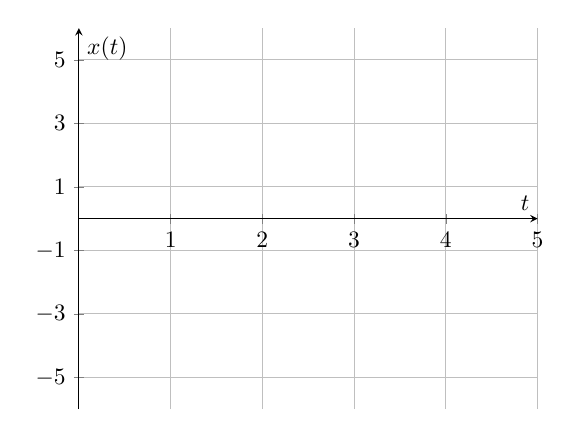
\begin{tikzpicture}[scale=0.85]
  \begin{axis}[
    xmin=0, xmax=5,
    ymin=-6, ymax=6,
    axis lines=middle,
    xlabel=$t$, ylabel={$x(t)$},
    xtick={0,1,2,3,4,5},
    ytick={-5,-3,-1,0,1,3,5},
    xticklabel style={anchor=north},
    yticklabel style={anchor=east},
    grid=both,
  ]
  \end{axis}
\end{tikzpicture}
\hspace{0cm}
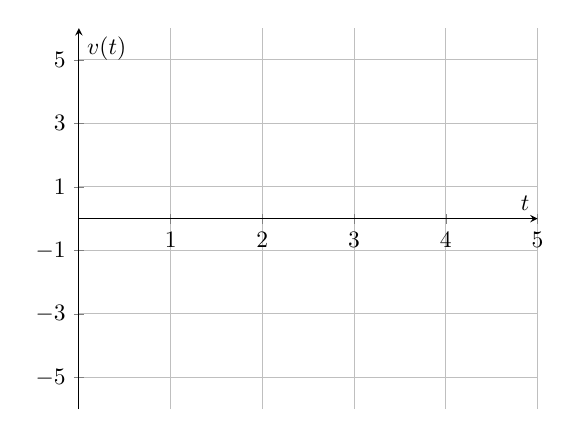
\begin{tikzpicture}[scale=0.85]
  \begin{axis}[
    xmin=0, xmax=5,
    ymin=-6, ymax=6,
    axis lines=middle,
    xlabel=$t$, ylabel={$v(t)$},
    xtick={0,1,2,3,4,5},
    ytick={-5,-3,-1,0,1,3,5},
    xticklabel style={anchor=north},
    yticklabel style={anchor=east},
    grid=both,
  ]
  \end{axis}
\end{tikzpicture}
\hspace{0cm}
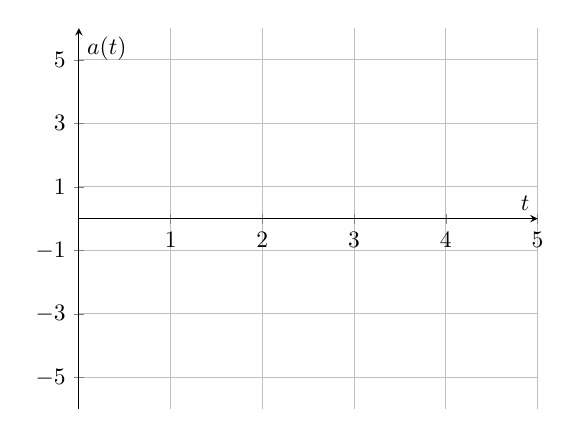
\begin{tikzpicture}[scale=0.85]
  \begin{axis}[
    xmin=0, xmax=5,
    ymin=-6, ymax=6,
    axis lines=middle,
    xlabel=$t$, ylabel={$a(t)$},
    xtick={0,1,2,3,4,5},
    ytick={-5,-3,-1,0,1,3,5},
    xticklabel style={anchor=north},
    yticklabel style={anchor=east},
    grid=both,
  ]
  \end{axis}
\end{tikzpicture}













\end{worksheet}

\end{document}